\documentclass[12pt, letterpaper]{article}

% ==========================================
%              DOCUMENT PACKAGES
% ==========================================

% --- Core Language & Encoding ---
\usepackage[english]{babel} % Sets the language and regional settings for English documents
\usepackage[utf8]{inputenc} % Allows the use of UTF-8 characters in the document
\usepackage[T1]{fontenc} % Specifies the font encoding
\usepackage[margin=2cm]{geometry} % Sets the page margins

% --- Colors & Graphics ---
\usepackage[table,dvipsnames]{xcolor} % Advanced color management
% \usepackage{color} % Basic package for text and background colors
\usepackage{graphicx} % Enhanced support for including external images and scaling them
\usepackage{adjustbox} % Adjusts the size, scaling, and alignment of boxes, images, and tables
% \usepackage{background} % Allows adding background images or watermarks to pages
\usepackage{float} % Improves the interface for floating objects and adds the [H] placement
\usepackage{pdflscape} % Makes landscape pages display correctly on screen in PDF viewers
\usepackage{pdfpages} % Allows the inclusion of external multi-page PDF documents

% --- Math, Science & Engineering ---
\usepackage{amsfonts} % Provides extended mathematical fonts
\usepackage{amsmath} % Provides advanced mathematical typesetting and environments
\usepackage{amssymb} % Provides extended mathematical symbols
% \usepackage{amsmath, amssymb} % (Redundant combination line omitted for stability)
\usepackage{amsthm} % Facilitates the creation of theorem-like environments
\usepackage{mathtools} % Enhances amsmath with additional math tools and bug fixes
\usepackage{thmtools} % Extensions and customization options for theorem environments
\usepackage{nicematrix} % Enhances matrices and tabulars using PGF/TikZ
\usepackage{xy} % Typesets complex graphs and diagrams
\usepackage{circuitikz} % Allows drawing of electrical networks and circuits

% --- Typography & Fonts ---
\usepackage{avant} % Sets the default sans-serif font to Avant Garde
\usepackage{cantarell} % Sets the default sans-serif font to Cantarell
\usepackage{charter} % Sets the default roman font to Charter
\usepackage{cmbright} % Sets the font family to Computer Modern Bright 
\usepackage{helvet} % Sets the default sans-serif font to Helvetica
\usepackage{inconsolata} % Sets the default typewriter (monospace) font to Inconsolata
\usepackage{iwona} % Sets the font family to Iwona 
\usepackage{kurier} % Sets the font family to Kurier 
\usepackage{lmodern} % Loads the Latin Modern fonts 
\usepackage{textcomp} % Provides additional text symbols
\usepackage{ulem} % Provides various types of text underlining and strikethroughs

% --- Tables & Lists ---
\usepackage{array} % Extends the array and tabular environments
\usepackage{arydshln} % Allows dashed lines in arrays and tables
\usepackage{bigstrut} % Adds custom vertical space in table rows
\usepackage{booktabs} % Enhances the quality of tables with better horizontal rules
% \usepackage{colortbl} % Allows coloring of rows, columns, and individual cells in tables
\usepackage{diagbox} % Creates table cells with diagonal lines
\usepackage{enumitem} % Provides advanced control over list environments
\usepackage{longtable} % Allows tables to break across multiple pages
\usepackage{multirow} % Allows individual table cells to span across multiple rows
\usepackage{tabularx} % Creates tables with dynamically adjustable-width columns
\usepackage{pgfplotstable} % Reads and cleanly formats numerical tables directly from CSV

% --- Formatting, Layout & UI ---
\usepackage{blindtext} % Generates dummy text for testing document layouts
\usepackage{caption} % Customizes captions in floating environments
\usepackage{comment} % Allows you to block out large sections of text
\usepackage{emptypage} % Automatically removes headers and footers on empty pages
\usepackage{fancyhdr} % Allows complete customization of headers and footers
\usepackage{fancyvrb} % Enhanced verbatim environments for writing raw code
\usepackage{framed} % Creates framed, shaded, or differently highlighted text regions
\usepackage{fullpage} % Quickly sets all page margins to 1 inch
\usepackage{lipsum} % Generates Lorem Ipsum dummy text
\usepackage{mdframed} % Creates highly customizable framed environments
\usepackage{multicol} % Allows intermixing single and multiple text columns
\usepackage{parskip} % Replaces standard paragraph indentation with vertical spacing
\usepackage{setspace} % Controls line spacing (single, one-and-a-half, double)
\usepackage{subcaption} % Supports sub-figures and sub-tables with independent captions
% \usepackage{subfig} % Older package for sub-figures (subcaption is generally preferred now)
\usepackage{tcolorbox} % Creates heavily customized colored and framed text boxes
\usepackage{titlesec} % Customizes the formatting of section, subsection, and chapter headings
\usepackage{titling} % Provides advanced control over the typesetting of the document title

% --- Bibliographies & References ---
\usepackage{biblatex} % Advanced, modern bibliographic processing and formatting
\usepackage{csquotes} % Context-sensitive quotation facilities
\usepackage{makeidx} % Supports the generation of a document index
% \usepackage{natbib} % Flexible bibliography support, particularly for author-year citation styles

% --- TikZ & Plotting ---
\usepackage{tikz} % Advanced package for creating vector graphics and diagrams programmatically
\usepackage{pgf-pie} % Draws pie charts programmatically using PGF/TikZ
\usepackage{pgfplots} % Creates high-quality mathematical plots, charts, and graphs
% \usepackage{fancytikzposter} % Used to create large format academic posters using TikZ

% --- URLs & Hyperlinks ---
\usepackage{url} % Formats and properly hyphenates long URLs
\usepackage{breakurl} % Allows line breaks in URLs, especially when compiled with latex -> dvips
\usepackage{hyperref} % Creates cross-referencing, clickable links, and PDF bookmarks

% --- Code Formatting ---
\usepackage{listings} % Typesets programming source code with formatting and syntax highlighting


% ==========================================
%           DOCUMENT CONFIGURATION
% ==========================================

% Custom color definitions
\definecolor{mygray}{gray}{0.9}

% Hyperlink configuration
\hypersetup{
    colorlinks=true,
    linkcolor=blue,
    urlcolor=blue
}

% Configuración adicional para breaks en URLs
\def\UrlBreaks{\do\/\do-\do_\do.\do=\do?\do\&}
\expandafter\def\expandafter\UrlBreaks\expandafter{\UrlBreaks\do\a\do\b\do\c\do\d\do\e\do\f\do\g\do\h\do\i\do\j\do\k\do\l\do\m\do\n\do\o\do\p\do\q\do\r\do\s\do\t\do\u\do\v\do\w\do\x\do\y\do\z}

%Uncomment the following lines to use a sans-serif font
%\renewcommand{\familydefault}{\sfdefault}

% TikZ libraries
\usetikzlibrary{shapes.geometric, positioning, decorations.pathreplacing}

\graphicspath{ {./img/} } % Sets the path for the graphics

\newlist{biblio}{enumerate}{1}
\setlist[biblio,1]{label=[\arabic*]}

\makeindex

% \tiny
% \scriptsize
% \footnotesize
% \small
% \normalsize (default size)
% \large
% \Large
% \LARGE
% \huge
% \Huge

% ==========================================
%         GLOBAL LISTINGS SETTINGS
% ==========================================
\lstset{
basicstyle=\ttfamily\small,
numbers=left,
numberstyle=\tiny\color{gray},
stepnumber=1,
numbersep=10pt,
backgroundcolor=\color{white},
showspaces=false,
showstringspaces=false,
breaklines=true,
frame=single,
tabsize=2,
captionpos=b,
lineskip=-1pt,
extendedchars=true,
literate={á}{{\'a}}1 {é}{{\'e}}1 {í}{{\'i}}1 {ó}{{\'o}}1 {ú}{{\'u}}1 {Á}{{\'A}}1 {É}{{\'E}}1 {Í}{{\'I}}1 {Ó}{{\'O}}1 {Ú}{{\'U}}1 {ñ}{{\~n}}1 {Ñ}{{\~N}}1 {¿}{{\textquestiondown}}1 {¡}{{\textexclamdown}}1
}

% ==========================================
%            LANGUAGE: SQL
% ==========================================
\lstdefinestyle{sqlstyle}{
	language=SQL,
	keywordstyle=\color{blue}\bfseries,
	commentstyle=\color[rgb]{0,0.5,0}\itshape,
	stringstyle=\color{red}
}

% ==========================================
%            LANGUAGE: VHDL
% ==========================================
\lstdefinelanguage{VHDL}{
	morekeywords={entity, architecture, signal, port, in, out, inout, begin, end, process, if, then, else, elsif, case, when, others, for, while, loop, wait, library, use, std_logic, std_logic_vector, integer, boolean, rising_edge, falling_edge, component, generic, map, downto, to, and, or, not, xor, nand, nor, xnor},
	morecomment=[l]{--},
	morestring=[b]",
	sensitive=false,
	alsoletter={_}
}

\lstdefinestyle{vhdl}{
	language=VHDL,
	keywordstyle=\color{blue}\bfseries,
	commentstyle=\color[rgb]{0,0.6,0}\itshape,
	stringstyle=\color{red}
}

% ==========================================
%              LANGUAGE: C
% ==========================================
\lstdefinestyle{cstyle}{
	language=C,
	keywordstyle=\color{blue}\bfseries,
	commentstyle=\color[rgb]{0,0.5,0}\itshape,
	stringstyle=\color{red},
	directivestyle=\color{purple},
	tabsize=4 % Overrides the global tabsize of 2 for C code specifically
}

% ==========================================
%             LANGUAGE: C++
% ==========================================
\lstdefinestyle{cppstyle}{
	language=C++,
	keywordstyle=\color{blue}\bfseries,
	commentstyle=\color[rgb]{0,0.5,0}\itshape,
	stringstyle=\color{red},
	directivestyle=\color{purple},
	tabsize=4
}

% ==========================================
%           LANGUAGE: PYTHON
% ==========================================
\lstdefinestyle{pythonstyle}{
	language=Python,
	keywordstyle=\color{blue}\bfseries,
	commentstyle=\color[rgb]{0,0.5,0}\itshape,
	stringstyle=\color{red},
	% Python relies heavily on indentation, so keeping tabsize aligned is important
	tabsize=4 }

% ==========================================
%             LANGUAGE: BASH
% ==========================================
\lstdefinestyle{bashstyle}{
	language=bash,
	keywordstyle=\color{blue}\bfseries,
	commentstyle=\color[rgb]{0,0.5,0}\itshape,
	stringstyle=\color{red},
	% Bash variables often use $, so we can highlight them dynamically if needed
	moredelim=[s][\color{orange}]{\$\{}{\}} }

% ==========================================
%           LANGUAGE: ASSEMBLY
% ==========================================
\lstdefinestyle{asmstyle}{
	language=[x86masm]Assembler,
	keywordstyle=\color{blue}\bfseries,
	commentstyle=\color[rgb]{0,0.5,0}\itshape,
	stringstyle=\color{red},
	% Adding common ARM/Microcontroller instructions for better highlighting
	morekeywords={ldr, str, mov, cmp, add, sub, b, bl, bx, push, pop, svc, eor,
			and, orr, lsl, lsr} }

% ==========================================
%          LANGUAGE: ARM / MICROPYTHON
% ==========================================
\lstdefinestyle{armstyle}{
	language=[x86masm]Assembler,
	keywordstyle=\color{blue}\bfseries,
	commentstyle=\color[rgb]{0,0.5,0}\itshape,
	stringstyle=\color{red},
	identifierstyle=\color{black},
	morekeywords={@micropython.asm_thumb, mov, cmp, add, sub, b, bhi, label, r0, r1, r2, r4},
	tabsize=4,
	basicstyle=\ttfamily\small
}

\newcommand{\numeroPractica}{2}
\newcommand{\tituloPractica}{Sistema de control de segundo orden}

%% Configure header
\setlength{\headheight}{28pt} % Adjust header height for two-line header
\pagestyle{fancy}
\fancyhf{} % Clear all header and footer fields
\lhead{\textbf{Nombre:} Ugartechea González Luis Antonio -- 320223822 \\ \textbf{Asignatura:} <asignatura>, \textbf{Grupo:} <grupo>}
\renewcommand{\headrulewidth}{0.4pt}

\begin{document}

\begin{titlepage}
	\providecommand{\numeroPractica}{1}
	\providecommand{\tituloPractica}{<titulo\_practica>}

	\begin{tikzpicture}[remember picture,overlay]
		\node[anchor=north west, inner sep=30] at (current page.north west) {
			
\includegraphics[width=3.5cm, height=4cm]{escudoUNAM_color.png}
		};
		% \node[anchor=north west, inner sep=30] at (current page.north west) {
		% 	
\includegraphics[width=4cm]{escudoUNAM_negro.png}
		% };

		\node[anchor=north east, inner sep=30] at (current page.north east) {
			
\includegraphics[width=3.5cm, height=4cm]{escudoFI_color.png}
		};
		% \node[anchor=north east, inner sep=30] at (current page.north east) {
		% 	
\includegraphics[width=4cm]{escudoFI_negro.png}
		% };
	\end{tikzpicture}

	\begin{center}
		\vspace*{2cm}

		\LARGE
		\textbf{Universidad Nacional Autónoma de México}\\
		Facultad de Ingeniería\\

		\vspace{1.5cm}

		\LARGE
		\textbf{Materia:} Organización Y Arquitectura de Computadoras\\
		\textbf{Profesor:} M.I. José Antonio de Jesús Arredondo Garza\\

		\vspace{1.5cm}

		\Huge
		\textbf{Práctica \numeroPractica}\\
		\LARGE
		\tituloPractica\\

		\vspace{1.5cm}

		\Large
		\begin{tabular}{|p{0.30\textwidth}|p{0.64\textwidth}|}
			\hline
			\textbf{No. de Cuenta} & \textbf{Nombre}                  \\
			\hline
			320068234              & Ayala Hernández María Fernanda   \\
			\hline
			320335163              & Salazar Islas Luis Daniel        \\
			\hline
			320078282              & Tepal Briseño Hansel Yael        \\
			\hline
			320223822              & Ugartechea González Luis Antonio \\
			\hline
		\end{tabular}
		\vspace{1cm}

		\LARGE
		\textbf{Fecha de entrega:} 12 de Octubre del 2026\\
		\vspace{0.5cm}
		\Huge
		\textbf{Calificación:} \underline{\hspace{3cm}}
		\vspace{2.5cm}
	\end{center}
\end{titlepage}


\section{Objetivo}

En esta práctica se implementó en una Raspberry Pi Pico 2 W un sistema de
control de segundo orden en tiempo discreto. El sistema lee la posición de un
potenciómetro mediante el convertidor analógico-digital (ADC), calcula la
salida usando una ecuación de diferencias y ejecuta el proceso cada $T_s=0.025\
    \mathrm{s}$, equivalente a una frecuencia de muestreo de $f_s=40\ \mathrm{Hz}$.

El objetivo es relacionar la función de transferencia continua con una
implementación digital en MicroPython y observar el comportamiento del sistema
directamente sobre el hardware.

\section{Fundamentos teóricos}

Una función de transferencia de segundo orden puede escribirse como
\begin{equation}
    H(s)=\frac{\omega_0}{s^2+2\omega_0s+\omega_0^2}.
\end{equation}
Para trabajar con la Raspberry Pi Pico 2 W, el sistema continuo debe
discretizarse para obtener una función $H(z)$ y una ecuación de diferencias.

El periodo de muestreo utilizado es
\begin{equation}
    T_s=0.025\ \mathrm{s},
    \qquad f_s=\frac{1}{T_s}=40\ \mathrm{Hz}.
\end{equation}

La implementación utiliza la forma discreta
\begin{equation}
    H(z)=\frac{b_0+b_1z^{-1}+b_2z^{-2}}
    {1+a_1z^{-1}+a_2z^{-2}}.
\end{equation}

Despejando la salida se obtiene la ecuación de diferencias
\begin{equation}
    y[k]=b_0x[k]+b_1x[k-1]+b_2x[k-2]
    -a_1y[k-1]-a_2y[k-2].
\end{equation}

En el programa se emplean los coeficientes
\begin{equation}
    b_0=0.01,\quad b_1=0.02,\quad b_2=0.01,
    \qquad a_1=-1.6,\quad a_2=0.64.
\end{equation}

Por tanto, el denominador queda como
\begin{equation}
    z^2-1.6z+0.64=(z-0.8)^2.
\end{equation}

Los polos tienen magnitud $0.8$, por lo que se encuentran dentro del círculo
unitario y el filtro discreto es estable. Además, la suma de los coeficientes
del numerador es igual a la evaluación del denominador en $z=1$, por lo que la
ganancia de corriente directa es aproximadamente uno.

\section{Desarrollo}

El programa se divide en cuatro tareas principales:
\begin{itemize}
    \item configurar el ADC del pin 26 para leer el potenciómetro;
    \item suavizar la lectura mediante un filtro exponencial;
    \item calcular la salida del sistema con la ecuación de diferencias;
    \item ejecutar las tareas periódicamente y mostrar la muestra actual.
\end{itemize}

El ADC de la Pico entrega valores entre 0 y 65535. Para reducir las variaciones
rápidas del potenciómetro se utiliza un filtro de promedio exponencial:
\begin{equation}
    x_f[k]=\alpha x_{ADC}[k]+(1-\alpha)x_f[k-1],
    \qquad \alpha=0.1.
\end{equation}

Un valor pequeño de $\alpha$ produce una lectura más suave, aunque también
incrementa el tiempo de respuesta ante cambios del potenciómetro.

\subsection{Estados del sistema}

Las variables \texttt{x\_k1} y \texttt{x\_k2} almacenan las dos entradas
anteriores, mientras que \texttt{y\_k1} y \texttt{y\_k2} almacenan las dos
salidas anteriores. Al terminar cada iteración, los estados se desplazan para
que estén disponibles en el siguiente periodo de muestreo.

\subsection{Temporizador e interrupción}

El temporizador se configura con un periodo de 25 ms:
\begin{lstlisting}[style=pythonstyle]
timer_muestreo.init(period=25,
					mode=Timer.PERIODIC,
					callback=iteracion_control)
\end{lstlisting}

Cada interrupción ejecuta \texttt{iteracion\_control}, lee el ADC, actualiza el
filtro y calcula la salida. La interrupción no imprime directamente en la
terminal: solo guarda la última muestra. El bucle principal se encarga de
imprimirla, evitando operaciones de salida dentro de la interrupción.

\subsection{Protecciones de estabilidad}

El programa verifica que la salida sea finita mediante \texttt{isfinite}. Si se
detecta \texttt{nan} o infinito, se reinician los estados de salida. También se
limita la salida al intervalo del ADC, $[-65535,65535]$, para evitar que una
condición anormal se propague al resto del sistema.

\section{Implementación en MicroPython}

El código completo utilizado en la Raspberry Pi Pico 2 W es el siguiente.

\lstinputlisting[style=pythonstyle, caption={Implementación del sistema de control}]{source/practica_02.py}

\section{Conexión del potenciómetro}

El potenciómetro se conecta entre 3.3 V y GND, y su terminal central se lleva
al pin ADC26. Para disminuir el ruido eléctrico se recomienda colocar un
capacitor de 100 nF entre ADC26 y GND, lo más cerca posible de la placa. Una
resistencia serie de aproximadamente 1 k$\Omega$ puede colocarse entre el
cursor del potenciómetro y el ADC para formar un filtro RC junto con el
capacitor.

La Pico y el potenciómetro deben compartir la misma referencia de tierra. No
debe aplicarse 5 V al ADC, ya que sus entradas trabajan con el nivel de 3.3 V.

\section{Ejecución en la Raspberry Pi Pico}

El programa se carga y ejecuta desde la carpeta \texttt{practica\_02} con:
\begin{lstlisting}[style=bashstyle]
../upload.sh source/practica_02.py
\end{lstlisting}

El script de carga verifica que el archivo exista, libera el puerto serial si
está ocupado, copia el programa a la Pico como \texttt{main.py} y lo ejecuta
mediante \texttt{mpremote}.

\lstinputlisting[style=bashstyle, caption={Script utilizado para cargar el programa}]{../upload.sh}

\section{Interfaz de monitoreo y graficación}

Para observar el comportamiento del sistema se desarrolló una interfaz en
Python que recibe las muestras de la Raspberry Pi Pico 2 W mediante el puerto
serial USB. El programa de la Pico envía una línea por muestra con el formato
\texttt{DATA,tiempo\_ms,entrada,salida}. La interfaz separa estos cuatro
campos, convierte la entrada y la salida a valores numéricos y los dibuja en
dos gráficas actualizadas en tiempo real.

La interfaz se ejecuta en la computadora, no en la Pico. Por esta razón, el
puerto serial debe quedar libre después de cargar el programa. El monitor se
inicia desde la carpeta \texttt{practica\_02} con:

\begin{lstlisting}[style=bashstyle]
python3 graficar_practica_02.py /dev/ttyACM0
\end{lstlisting}

La ventana permite conectar y desconectar el puerto, pausar la visualización,
limpiar el historial y guardar las muestras recibidas en un archivo CSV. El
programa completo de la interfaz es el siguiente:

\lstinputlisting[style=pythonstyle, caption={Interfaz Python para graficar la entrada y la salida}]{graficar_practica_02.py}

\section{Resultados}

Al iniciar el programa se muestra el mensaje de arranque y después se envía una
línea serial por cada muestra:
\begin{lstlisting}[style=bashstyle]
Sistema de control de segundo orden iniciado a 40 Hz...
DATA,tiempo_ms,entrada,salida
\end{lstlisting}

La lectura se actualiza nominalmente cada 25 ms. El filtro EMA reduce las
variaciones rápidas del potenciómetro y los polos de magnitud 0.8 evitan el
crecimiento de la respuesta. La señal \texttt{x[k]} corresponde a la entrada
filtrada del ADC, mientras que \texttt{y[k]} es la salida calculada mediante la
ecuación de diferencias; no representa una tensión medida en un pin de salida.

\subsection{Pruebas con diferentes coeficientes}

Para comparar la respuesta del sistema se realizaron tres pruebas. En cada caso
se modificaron los coeficientes del programa, se volvió a cargar el firmware en
la Pico y se guardó una captura de la interfaz. Las imágenes deben colocarse en
la carpeta \texttt{practica\_02/img/} con los nombres indicados.

\begin{table}[H]
    \renewcommand{\arraystretch}{1.2}
    \centering
    \begin{tabular}{|c|ccc|cc|l|}
        \hline
        \rowcolor{black!80}
        \textcolor{white}{Prueba} & \textcolor{white}{$b_0$} & \textcolor{white}{$b_1$} & \textcolor{white}{$b_2$} & \textcolor{white}{$a_1$} & \textcolor{white}{$a_2$} & \textcolor{white}{Comportamiento} \\
        \hline
        1 & 0.010 & 0.020 & 0.010 & -1.6  & 0.64  & Respuesta base \\
        2 & 0.040 & 0.080 & 0.040 & -1.2  & 0.36  & Más rápida y amortiguada \\
        3 & 0.005 & 0.010 & 0.005 & -1.8  & 0.81  & Más lenta \\
        \hline
    \end{tabular}
    \caption{Coeficientes utilizados en las pruebas experimentales.}
    \label{tab:coeficientes-pruebas}
\end{table}

\begin{figure}[H]
    \centering
    \IfFileExists{img/grafica_01.png}{%
        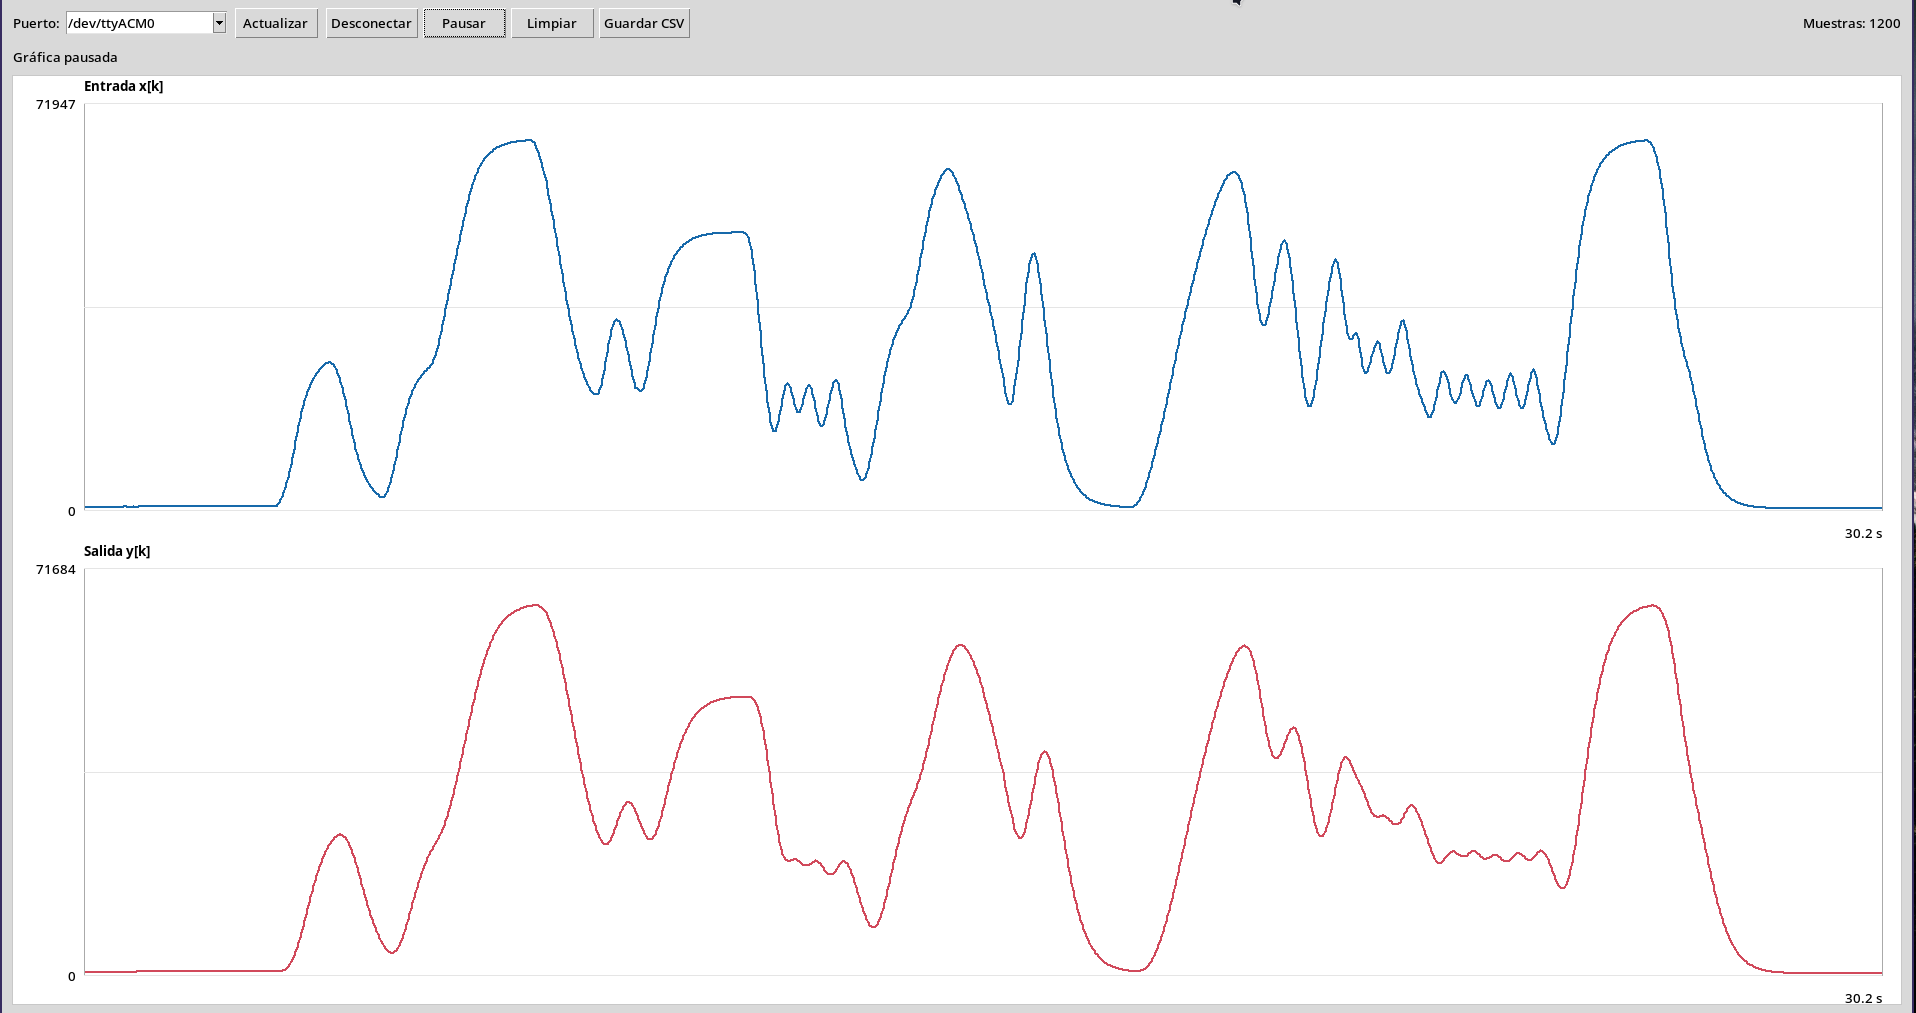
\includegraphics[width=\textwidth]{grafica_01.png}%
    }{%
        \fbox{\parbox[c][4cm][c]{0.85\textwidth}{\centering Insertar aquí \texttt{img/grafica\_01.png}}}%
    }
    \caption{Respuesta del sistema con los coeficientes de la prueba 1.}
    \label{fig:grafica-prueba-1}
\end{figure}

\begin{figure}[H]
    \centering
    \IfFileExists{img/grafica_02.png}{%
        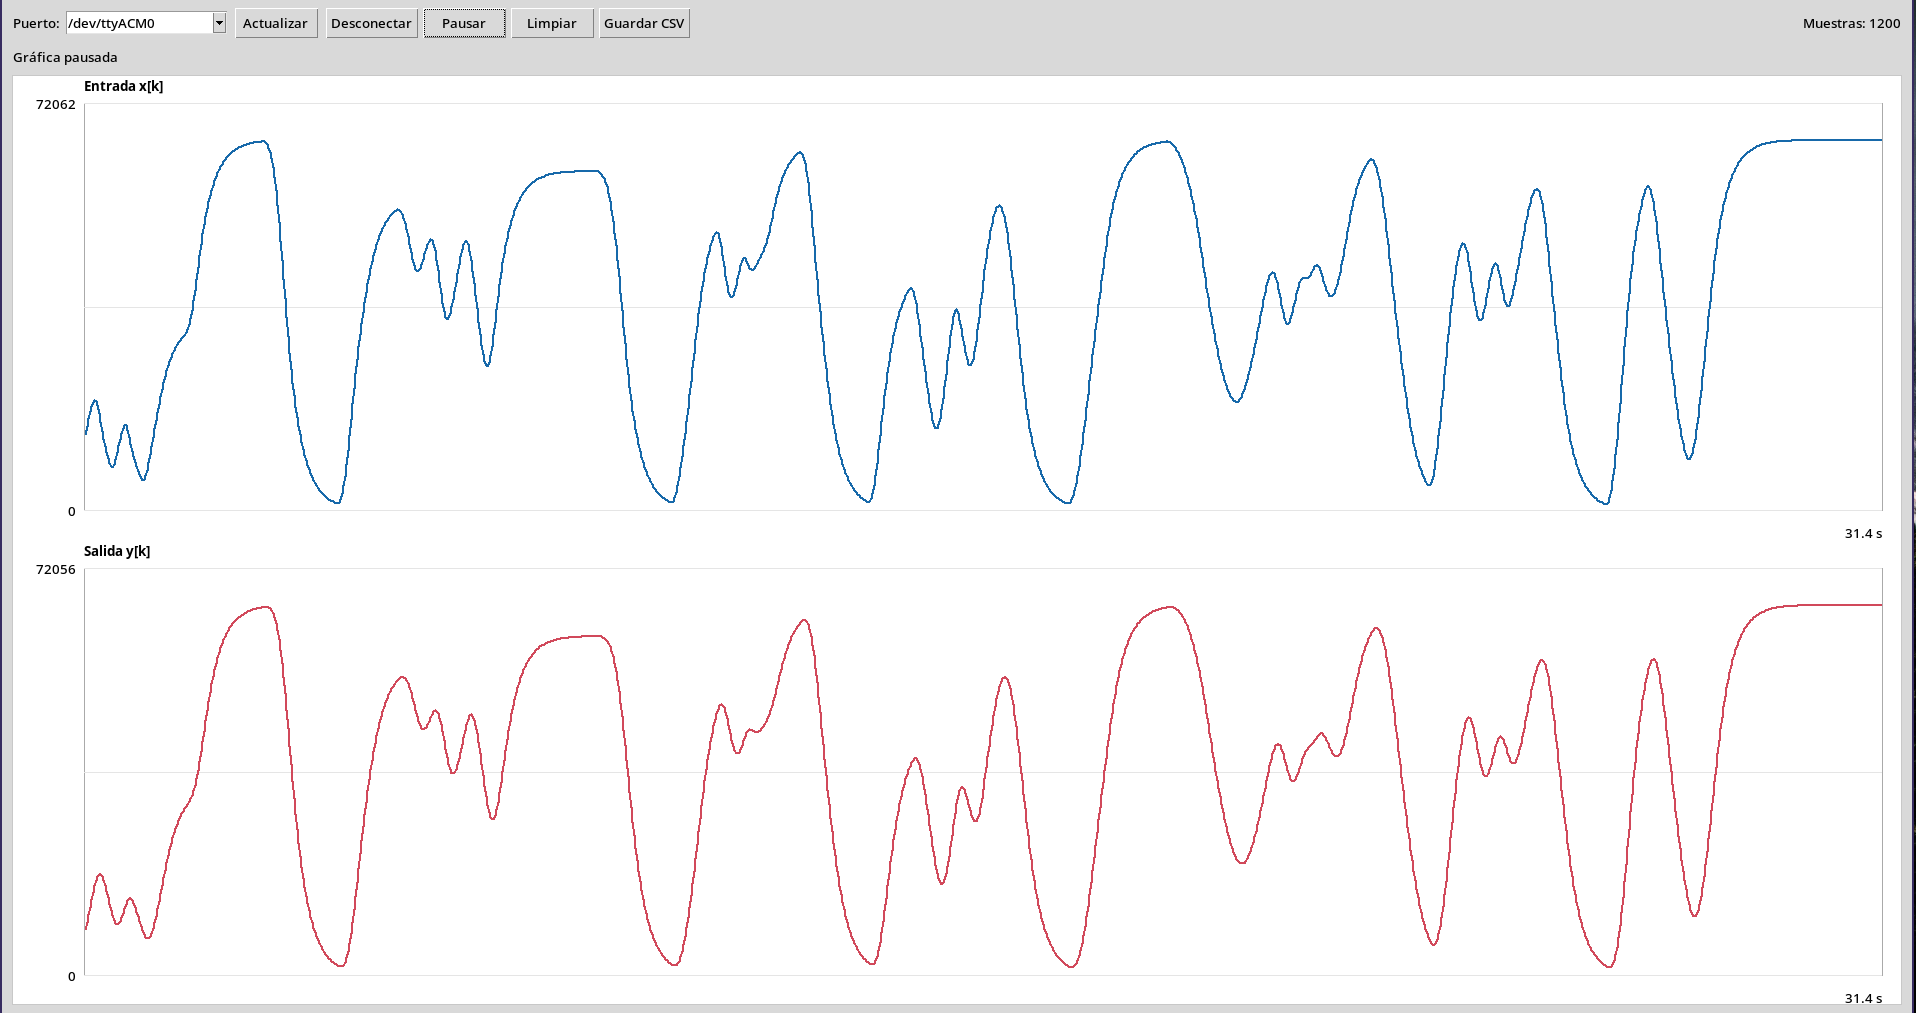
\includegraphics[width=\textwidth]{grafica_02.png}%
    }{%
        \fbox{\parbox[c][4cm][c]{0.85\textwidth}{\centering Insertar aquí \texttt{img/grafica\_02.png}}}%
    }
    \caption{Respuesta del sistema con los coeficientes de la prueba 2.}
    \label{fig:grafica-prueba-2}
\end{figure}

\begin{figure}[H]
    \centering
    \IfFileExists{img/grafica_03.png}{%
        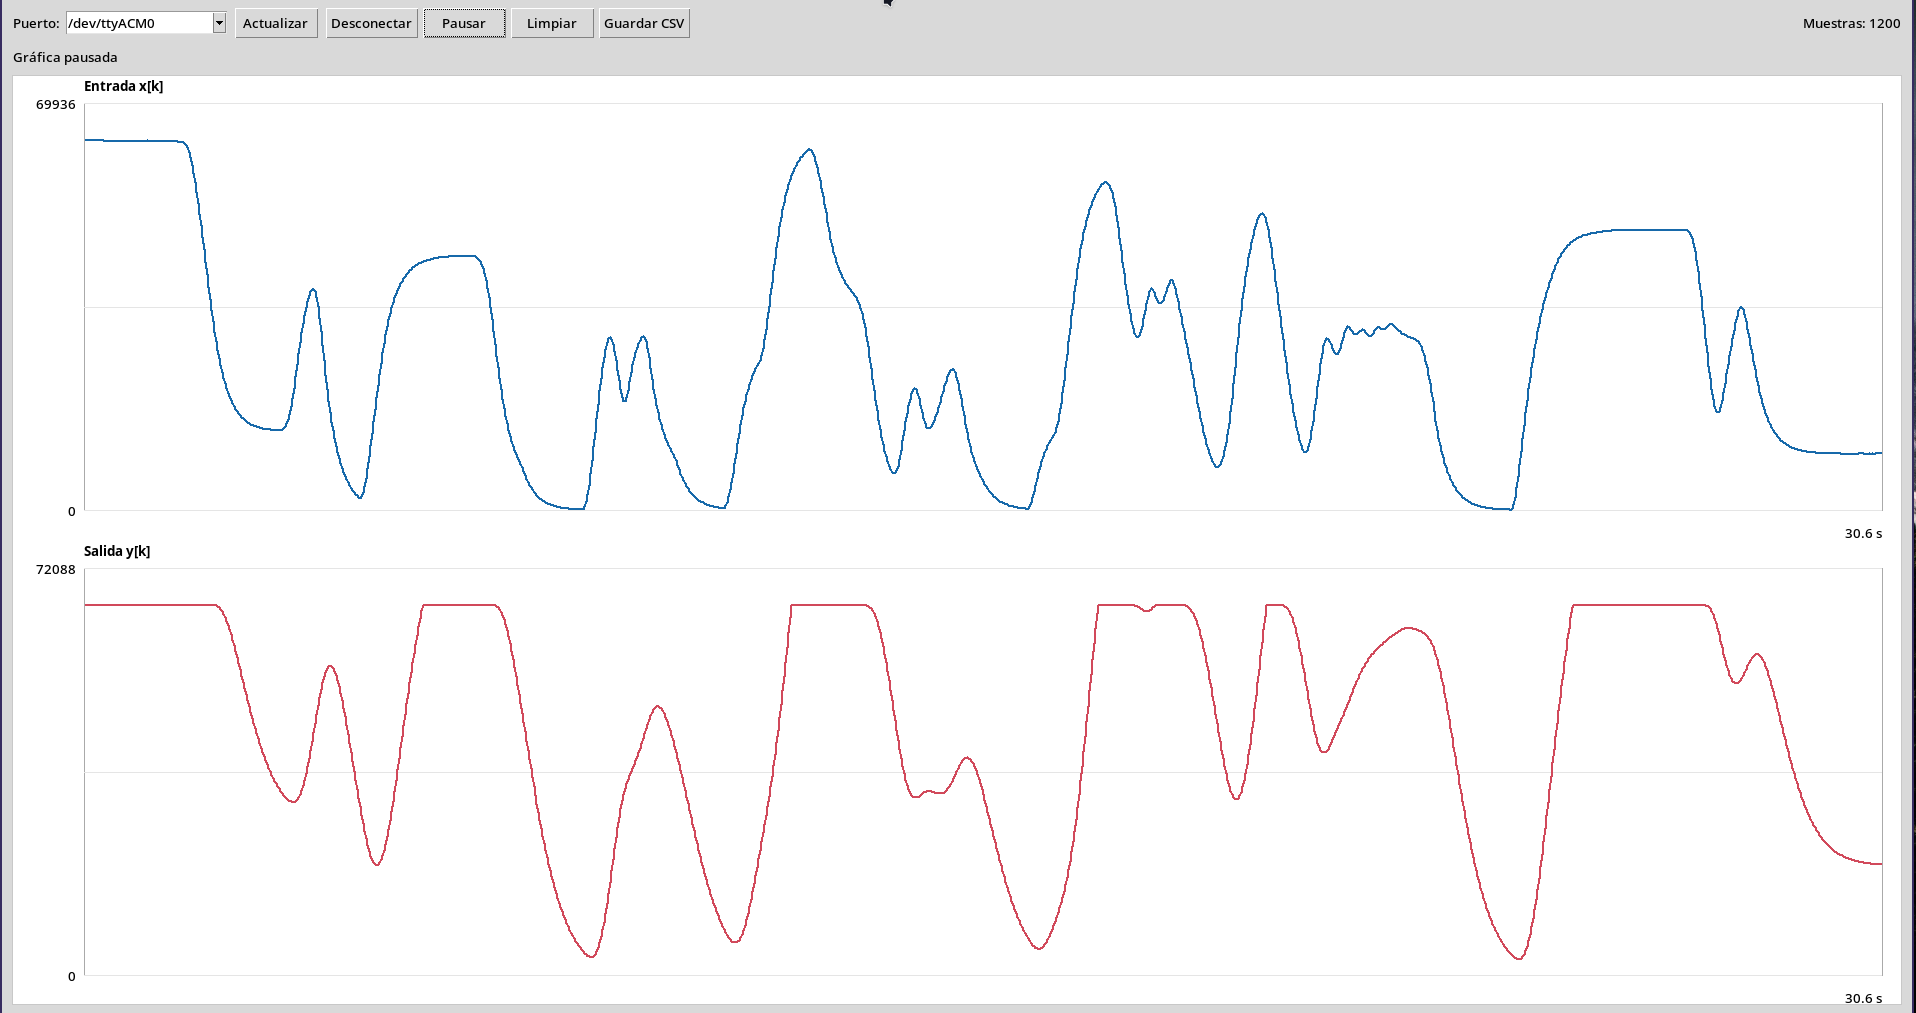
\includegraphics[width=\textwidth]{grafica_03.png}%
    }{%
        \fbox{\parbox[c][4cm][c]{0.85\textwidth}{\centering Insertar aquí \texttt{img/grafica\_03.png}}}%
    }
    \caption{Respuesta del sistema con los coeficientes de la prueba 3.}
    \label{fig:grafica-prueba-3}
\end{figure}

Las tres pruebas confirmaron que la posición de los polos modifica directamente la rapidez de respuesta del sistema. Los polos de magnitud 0.6 produjeron la respuesta más rápida, los polos de magnitud 0.8 produjeron una respuesta intermedia y los polos de magnitud 0.9 produjeron la respuesta más lenta. En los tres casos el sistema permaneció estable porque los polos se mantuvieron dentro del círculo unitario.

La salida también puede almacenarse en un archivo desde la terminal:
\begin{lstlisting}[style=bashstyle]
../upload.sh source/practica_02.py >> source/output.txt
\end{lstlisting}

\section{Conclusiones individuales}

\subsection{Ayala Hernández María Fernanda}

La práctica permitió implementar un sistema de segundo orden en tiempo discreto
sobre una Raspberry Pi Pico 2 W. El uso del ADC y del temporizador mostró cómo
un microcontrolador puede adquirir señales y procesarlas con un periodo de
muestreo definido.

\subsection{Salazar Islas Luis Daniel}

La implementación permitió relacionar una función de transferencia con una
ecuación de diferencias ejecutable en MicroPython. También se observó que la
elección de los polos es fundamental para evitar que la respuesta digital sea
inestable.

\subsection{Tepal Briseño Hansel Yael}

El filtrado exponencial ayudó a reducir el ruido producido por el
potenciómetro. Esta práctica mostró que la estabilidad depende tanto del
algoritmo de control como de la calidad de la señal de entrada y de la conexión
física del circuito.

\subsection{Ugartechea González Luis Antonio}

La ejecución en la Raspberry Pi Pico 2 W permitió comprobar la interacción
entre el software y el hardware. El temporizador periódico garantiza el ritmo
de procesamiento, mientras que la salida en la terminal facilita observar el
comportamiento del sistema durante las pruebas.

%\section{Bibliografía}

\begin{biblio}
	% for: https://sistemasmultibasededatos.blogspot.com/
	\item Esquivel Martinez H. (2021, Noviembre 28). \textit{SISTEMAS MULTIBASE DE DATOS} [Online]. Disponible en: \newline \url{https://sistemasmultibasededatos.blogspot.com/}
\end{biblio}

\end{document}
